\documentclass[fontsize=12pt]{scrartcl}
\usepackage[ngerman]{babel}
\usepackage[utf8]{inputenc}
%\usepackage[latin1]{inputenc}
\usepackage{amsmath}
\usepackage{amstext}
\usepackage{amssymb}
\usepackage{stmaryrd}
\usepackage{verbatim}
\usepackage{mathrsfs}
\usepackage{extarrows}
\usepackage[arrow, matrix, curve]{xy}
\usepackage[centering,includeheadfoot,margin=2cm]{geometry}
\usepackage{gensymb}
\usepackage{graphicx}
\usepackage{framed}
\usepackage{tabularx}
\usepackage{xcolor}
\usepackage{float}
\usepackage{graphicx} 
\usepackage{sidecap}
\usepackage{blindtext,wrapfig}
\usepackage{epstopdf}
\usepackage{import}
\usepackage{fancyhdr}
\usepackage{fancybox}
\usepackage{paralist}
\usepackage{graphicx}
\usepackage{caption}
\usepackage{subcaption}
\renewcommand{\l}{\left\vert}
\renewcommand{\r}{\right\vert}
\newcommand{\define}{\ensuremath{\mathrel{\mathop:}=}} % hübscheres :=, da = zentriert wird relativ zu :
\newcommand{\enifed}{\ensuremath{=\mathrel{\mathop:}}} % hübscheres =:, da = zentriert wird relativ zu :
\newcommand{\ddt}{\frac{\partial}{\partial t}}
\newcommand{\ddn}{\frac{\partial}{\partial N}}
\DeclareGraphicsRule{.tif}{png}{.png}{`convert #1 `basename #1 .tif`.png} 
\pagestyle{fancy}
\fancyhf{}
\fancyhead[R]{Physikalisches Praktikum 1}
\fancyfoot[R]{\thepage}
\fancyfoot[L]{\today}
\fancyhead[L]{Gentian Rrafshi}
\parindent 0pt
\parskip 12pt
\begin{document}

\begin{minipage}{0.9\textwidth}
\begin{center}\large
\title{ W43 Messung des Adiabatenexponenten \\
		~\\
		~\\
		Assistent: Charlot Riedmüller \\
		Datum Versuchsdurchführung: \\
		24.09.2015}

\author{bearbeitet von\\
		Gruppe: \\
		Gentian Rrafshi Matrnr. 2721617}
\date{\today}

\maketitle

\end{center}
\end{minipage}

\newpage

\tableofcontents

\newpage
\noindent

\section{ Versuchsziel}

Ziel des Versuchs ist die Messung des Adiabatenexponenten von Luft, Kohlenstoffdioxid (CO$_2$) und Argon (Ar) mit Hilfe der Gasfeder.

\section{ Grundlagen}

Grundlage dieses Versuchs ist der adiabate Prozess. Dieser geschieht genau dann, wenn ein Im Vorgang kein Wärmeaustausch stattfindet. \par

Da kein Wärmeaustausch stattfindet, ist ist $\Delta Q =0$, was mit Hilfe des ersten Hauptsatzes der Thermodynamik
\begin{equation}
\Delta U = \Delta Q + \Delta W
\end{equation}
als Konsequenz 
\begin{equation}
\Delta U =  \Delta W
\end{equation}
mit sich zieht. Damit ist die innere Energie gleich der verrichteten Arbeit. \par

Der adiabate Prozess ist ein rein theoretischer Vorgang und taucht so nicht in der Natur auf. Es gibt allerdings Vorgänge, die annähernd Adiabat sind. Beispielhaft wäre da die Thermoskanne, bei Kompression einer Luftpumpe und generell alles, was als \glqq Wärmedicht \grqq bezeichnet wird. \par

Es wird im allgemeinen zwischen irreversiblen und reversiblen Kreisprozessen unterschieden. \par

Die Besonderheit hierbei liegt an der Entropie. Ist der Vorgang reversibel, so nennt man den adiabate Zustandsänderung auch Isentrope Zustandsänderung. Zudem heißt dies auch, des bei reversiblen Prozessen auch keine Entropie dem Vorgang zugeführt wird. Daher bleibt die Entropie konstant. \par

Bei irreversiblen Vorgängen heißt dies, dass dem System Entropie zugeführt wird. Solche irreversiblen Vorgänge laufen meist spontan ab, wie zum Beispiel beim Temperaturausgleich. 

Eine weitere Grundlage dieses Versuchs bildet die Wärmekapazität eines Körpers, welches das Verhältnis der ihm zugeführten Wärme zu der damit bewirkten Temperaturerhöhung ist. Formal also:
\begin{align*}
C=\frac{\text{d}Q}{\text{d}T}
\end{align*}
Wobei $\text{d}Q$ die zugeführte Wärme und $\text{d}T$ die bewirkte Temperaturerhöhung ist. \par
\newpage
Weiterführend zur Wärmekapazität betrachtet man die spezifische Wärmekapazität, welche angibt wie viel Wärme ein Stoff bei Temperaturänderungen pro Masseneinheit aufnimmt bzw. abgibt. Es gilt also:
\begin{align*}
c_{\text{spez}}=\frac{\text{d}Q}{m\cdot \text{d}T}
\end{align*}
Hieraus ergibt sich der Isentropenexponent bzw. Adiabatenexponent. Dieser ist das Verhältnis bei Gasen zwischen der (spezifischen) Wärmekapazität bei konstantem Druck ($c_p$) und konstanten Volumen ($c_V$). Formal gilt also:
\begin{align*}
\kappa = \frac{c_p}{c_V}
\end{align*}
Weiterführend gilt als gute Annäherung, dass
\begin{align*}
\kappa = \frac{f+2}{f}
\end{align*}
gilt. Hierbei ist $f$ nun die Anzahl der Freiheitsgrade, welches ein System besitzt (in diesem Fall Moleküle und Atome). \par
Mit Hilfe des Adiabatenexponenten kann man nun die Adiabatengleichungen für Gase in der adiabaten Zustandsänderung definieren, welche wie folgt lauten:
\begin{align*}
pV^{\kappa} = const. \\
T^{\kappa}p^{1-\kappa} = const. \\
TV^{\kappa-1}=const.
\end{align*}
Wobei hier $T$ für die Temperatur, $V$ für das Volumen und $p$ für den Druck stehen.
\newpage

\section{Versuchsdurchführung}

\begin{figure}[H]
\centering
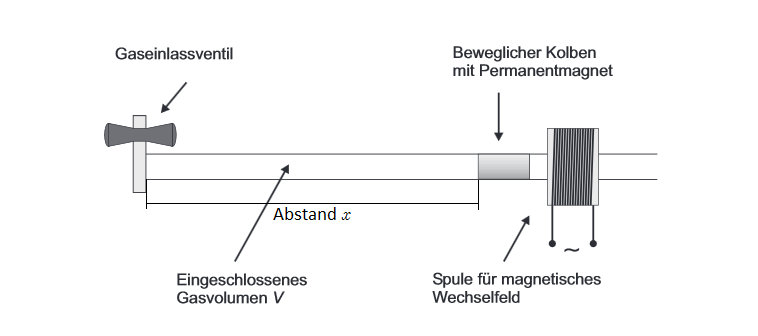
\includegraphics[width=0.75\textwidth]{Graphik/W43}
\label{43}
\caption{Versuchsskizze$^{\cite{A}}$}
\end{figure}

Um den Adiabatenexponent $\gamma$ für Luft, Kohlenstoffdioxid (CO$_2$) und Argon (Ar) zu bestimmen, benötigen wir ein horizontal gelagertes Glasrohr. In diesem Glasrohr ist ein Kolben mit einem Eisenkern, welcher durch einen Permanentmagnet von außen verschoben werden kann. \par

Auf einer Seite des Glasrohrs ist ein Ventil eingebracht. Durch dieses Ventil kann Gas rein-, rausgelassen und eingeschlossen werden.
Mit dem Permanentmagneten lässt sich der Kolben auf eine gewünschten Position hinpositioniert werden. Dieser Abstand $x$ vom Ventil zum Kolben soll notiert werden. wird notiert.
Das dadurch eingeschlossene Gas verhält sich nun, wenn der Kolben mit Hilfe der Spule in Schwingung versetzt wird,  analog zu einer Feder beim Federpendel.\par

Durch einen Drehzahlregler soll nun der Kolben so in Schwingung versetzt werden, dass der Kolben den maximal möglichen Ausschlag hat. 
Diese Frequenz ist dann die Eigenfrequenz des Systems und soll notiert werden. Im Anschluss wird noch der neue Abstand notiert, nach dem der Kolben wieder in Ruhe ist. Dies wird jeweils drei mal für Luft, CO$_2$ und Argon ausgeführt.


\noindent
\newpage


\section{Formeln}

Für den Versuch ist nur eine Formel relevant:
\begin{equation}
\gamma = \frac{16\pi \cdot m \cdot x \cdot f}{d_{\text{Rohr}}^2 \cdot p_0}
\label{1}
\end{equation}
Hierbei sind $m$ = $8,8781\cdot 10^{-3}$\,kg, $p_0$ = $1,021\cdot 10^{5}$\,Pa und $d_{\text{Rohr}}= 16$\,mm. Desweiteren sind $p_0$ der Luftdruck, $x$ der Abstand wie in Abbildung (1) eingezeichnet und $f$ die gemessene Frequenz.

\section{ Messwerte}
\begin{figure}[H]
\centering
\caption{Messwerte für Luft}
\begin{tabular}{|c|c|c|} \hline
Abstand davor $x$ [cm]	& Abstand danach $x$ [cm] & $f$ [Hz]\\ \hline
30,00&	30,40&	15,60 \\ \hline
20,00&	19,60&	19,50\\ \hline
10,00&	9,90&	27,00\\ \hline
\end{tabular}				 
\end{figure}
\begin{figure}[H]
\centering
\caption{Messwerte für CO$_2$}
\begin{tabular}{|c|c|c|} \hline
Abstand davor $x$ [cm]	& Abstand danach $x$ [cm] & $f$ [Hz]\\ \hline
22,50&	22,00&	17,70\\ \hline
28,00&	27,60&	15,70\\ \hline
46,00&	45,50&	12,00\\ \hline
\end{tabular}				 
\end{figure}
\begin{figure}[H]
\centering
\caption{Messwerte für Argon}
\begin{tabular}{|c|c|c|} \hline
Abstand davor $x$ [cm]	& Abstand danach $x$ [cm] & $f$ [Hz]\\ \hline
27,50&	27,80&	17,70\\ \hline
39,50&	40,50&	14,50\\ \hline
10,30&	10,50&	28,00\\ \hline
\end{tabular}				 
\end{figure}
\newpage

\section{ Auswertung}

Mit Hilfe der Formel (\ref{1}) kann man nun den Adiabatenexponenten $\gamma$ bestimmen. Dazu eine kleine Beispielrechnung für Luft bei 30,4\,cm Abstand. Die übrigen Werte werden dann tabellarisch aufgelistet.
\begin{align*}
\gamma = \frac{16\pi \cdot m \cdot x \cdot f}{d_{\text{Rohr}}^2 \cdot p_0} = \frac{16\cdot\pi \cdot 8,8781 \cdot 10^{-3}\text{kg} \cdot 0,304\text{m} \cdot (15,6 \text{s}^{-1})^2}{(1,6 \cdot 10^{-2}\text{m})^2 \cdot 1,021 \cdot 10^5 \frac{\text{N}}{\text{m}^2}} = 1,26
\end{align*}

\begin{figure}[H]
\centering
\caption{Ergebnisse für Luft}
\begin{tabular}{|c|c|c|c|} \hline
Abstand davor $x$ [cm]	& Abstand danach $x$ [cm] & $f$ [Hz] & $\gamma$ \\ \hline
30,00&	30,40&	15,60&	1,26	 \\ \hline
20,00&	19,60&	19,50&	1,27	\\ \hline
10,00&	9,90&	27,00&		1,23 	\\ \hline
\end{tabular}				 
\end{figure}
\begin{figure}[H]
\vspace{-24pt}
\centering
\caption{Ergebnisse für CO$_2$}
\begin{tabular}{|c|c|c|c|} \hline
Abstand davor $x$ [cm]	& Abstand danach $x$ [cm] & $f$ [Hz] & $\gamma$\\ \hline
22,50&	22,00&	17,70&	1,18	\\ \hline
28,00&	27,60&	15,70&	1,16	\\ \hline
46,00&	45,50&	12,00&	1,12	\\ \hline
\end{tabular}				 
\end{figure}
\begin{figure}[H]
\vspace{-24pt}
\centering
\caption{Ergebnisse für Argon}
\begin{tabular}{|c|c|c|c|} \hline
Abstand davor $x$ [cm]	& Abstand danach $x$ [cm] & $f$ [Hz] & $\gamma$\\ \hline
27,50&	27,80&	17,70	& 1,49	\\ \hline
39,50&	40,50&	14,50	&	1,45 \\ \hline
10,30&	10,50&	28,00	&	1,40 \\ \hline
\end{tabular}				 
\end{figure}

Gemittelt ergibt sich also folgendes:
\begin{itemize}
\centering
\item[] $\bar{\gamma}_{\text{Luft}}$ =1,26 \hspace{50pt} Literaturwert $\gamma_{\text{Luft}}$ =1,4
\item[] $\bar{\gamma}_{\text{CO}_2}$ =1,15 \hspace{50pt} Literaturwert $\gamma_{\text{CO}_2} =1,\bar{3}$
\item[] $\bar{\gamma}_{\text{Ar}}$ =1,45 \hspace{50pt} Literaturwert $\gamma_{\text{Ar}} =1,\bar{6}$
\end{itemize}

\newpage
\section{Fehlerrechnung}

Folgende Fehler wurden dem Versuch entnommen:
\begin{itemize}
\item Außendruck (Luftdruck) $\Delta $p$_0= 0, 002\cdot 10^5\,\frac{\text{N}}{\text{m}^2}$
\item Masse des Oszillators $\Delta $m$= 0, 0001$\,g
\item Durchmesser des Glasrohrs $\Delta $d$_{\text{Rohr}}=0, 01$\,mm
\end{itemize}
Desweiteren werden diese Fehler angenommen:
\begin{itemize}
\item Abstand  $\Delta $x$= 1\cdot 10^{-3}\,\text{m}$
\item Frequenz $\Delta $f$= 0,5$\,Hz
\end{itemize}

Mit Hilfe der Fehlerfortpflanzung ergibt sich folgender Fehler für $\gamma$:
\begin{align*}
\Delta \gamma &= \l \frac{\partial}{\partial m} \gamma \r \cdot \Delta m + \l \frac{\partial}{\partial x} \gamma \r \cdot \Delta x+ \l \frac{\partial}{\partial f} \gamma \r \cdot \Delta f +\l \frac{\partial}{\partial d_{\text{Rohr}}} \gamma \r \cdot \Delta d_{\text{Rohr}}+ \l \frac{\partial}{\partial p_{0}} \gamma \r \cdot \Delta p_{0}\\
~\\
&= 16\pi (\frac{x f^2 \Delta m + m f^2 \Delta x + 2mx\Delta f}{d_{\text{Rohr}}^2 \cdot p_0} +\frac{ 2mx f^2 \Delta d_{\text{Rohr}} }{d_{\text{Rohr}}^3 \cdot p_0} + \frac{ 2mx f^2 \Delta  p_0 }{d_{\text{Rohr}}^2 \cdot p_0^2})
\end{align*}

Da einer Beispielrechnung hier sehr unübersichtlich wird, werden die Ergebnisse gleich in den nachfolgenden Tabellen angegeben:

\begin{figure}[H]
\centering
\caption{Fehler für Luft}
\begin{tabular}{|c|c|c|c|} \hline
 $\gamma$  & Fehler  $\Delta \gamma$\\ \hline
1,26	&0,12	\\ \hline
1,27	&0,18	\\ \hline
1,23	&0,33	\\ \hline
\end{tabular}				 
\end{figure}
\begin{figure}[H]
\vspace{-24pt}
\centering
\caption{Fehler für CO$_2$}
\begin{tabular}{|c|c|c|c|} \hline
 $\gamma$ & Fehler  $\Delta \gamma$\\ \hline
1,18	&0,15	\\ \hline
1,16	&0,12	\\ \hline
1,12	&0,08	\\ \hline
\end{tabular}				 
\end{figure}
\begin{figure}[H]
\vspace{-24pt}
\centering
\caption{Fehler für Argon}
\begin{tabular}{|c|c|c|c|} \hline
 $\gamma$ & Fehler  $\Delta \gamma$ \\ \hline
1,49	&0,15	\\ \hline
1,45	&0,11	\\ \hline
1,40	&0,36	\\ \hline
\end{tabular}				 
\end{figure}

Als hat man folgende Fehler:
\begin{itemize}
\centering
\item[] $\Delta\bar{\gamma}_{\text{Luft}} = 0,33$ 
\item[] $\Delta \bar{\gamma}_{\text{CO}_2} = 0,15$
\item[] $\Delta \bar{\gamma}_{\text{Ar}} =0,36$ 
\end{itemize}


\section{Zusammenfassung}

Ziel dieses Versuchs ist die Bestimmung des Adiabatenexponenten von Luft, Kohlenstoffdioxid (CO$_2$) und Argon (Ar). Zusammenfassend werden hier noch einmal alle wichtigen Ergebnisse aufgelistet:
\begin{figure}[H]
\centering
\caption{Ergebnisse für Luft}
\begin{tabular}{|c|c|c|c|} \hline
 Abstand danach $x$ [cm] & $f$ [Hz] & $\gamma$ & Fehler  $\Delta \gamma$ \\ \hline
0,30	&15,60	&1,26	&0,12	\\ \hline
0,20	&19,50	&1,27	&0,18	\\ \hline
0,10	&27,00	&1,23	&0,33	\\ \hline
\end{tabular}				 
\end{figure}
\begin{figure}[H]
\vspace{-24pt}
\centering
\caption{Ergebnisse für CO$_2$}
\begin{tabular}{|c|c|c|c|} \hline
 Abstand danach $x$ [cm] & $f$ [Hz] & $\gamma$ & Fehler  $\Delta \gamma$\\ \hline
0,22	&17,70	&1,18	&0,15	\\ \hline
0,28	&15,70	&1,16	&0,12	\\ \hline
0,46	&12,00	&1,12	&0,08	\\ \hline
\end{tabular}				 
\end{figure}
\begin{figure}[H]
\vspace{-24pt}
\centering
\caption{Ergebnisse für Argon}
\begin{tabular}{|c|c|c|c|} \hline
 Abstand danach $x$ [cm] & $f$ [Hz] & $\gamma$ & Fehler  $\Delta \gamma$\\ \hline
0,28	&17,70	&1,49	&0,15	\\ \hline
0,41	&14,50	&1,45	&0,11	\\ \hline
0,11&	28,00	&1,40	&0,36	\\ \hline
\end{tabular}				 
\end{figure}
Gemittelt bekommt man dadurch folgende Adiabatenexponenten:
\begin{itemize}
\centering
\item[] $\bar{\gamma}_{\text{Luft}} =1,26\pm 0,33$ \hspace{50pt} Literaturwert $\gamma_{\text{Luft}}$ =1,4
\item[] $\bar{\gamma}_{\text{CO}_2} =1,15\pm 0,15$ \hspace{50pt} Literaturwert $\gamma_{\text{CO}_2} =1,\bar{3}$
\item[] $\bar{\gamma}_{\text{Ar}}=1,45\pm 0,36$ \hspace{50pt} Literaturwert $\gamma_{\text{Ar}} =1,\bar{6}$
\end{itemize}
\newpage
\section{Literaturverzeichnis}

\renewcommand{\refname}{~}
\vspace{-30pt}
\begin{thebibliography}{xx}

   \bibitem[1]{1}  	\textit{\glqq  W43 Messung des Adiabatenexponenten\grqq , in 	\\
   					http://www3.physik.uni-stuttgart.de/studium/praktika/ap/}, \\
   					unter \textit{http://www3.physik.uni-stuttgart.de/studium/praktika/ap/pdf\_dateien/W43.pdf}; \\
   								abgerufen am 06.10.2015

   \bibitem[A]{A}  	Graphik aus \textit{\glqq  W43 Messung des Adiabatenexponenten\grqq , in 	\\
   					http://www3.physik.uni-stuttgart.de/studium/praktika/ap/}, \\
   					unter \textit{http://www3.physik.uni-stuttgart.de/studium/praktika/ap/pdf\_dateien/W43.pdf}; \\
   								abgerufen am 06.10.2015
\end{thebibliography}

\section{Anhang}

\end{document}